\documentclass[12pt,bibtotoc]{scrreprt}

% satz nach der norm auf der tu-seite

% referenzenh
\usepackage{cite}
\usepackage{bibgerm}

% farben definieren
\usepackage{xcolor}
\definecolor{lightblue}{cmyk}{0.346, 0.114, 0, 0.106}


% zeilenabstand (nach dem dokument auf der tu-seite)
\usepackage[onehalfspacing]{setspace}

% deutsch
\usepackage{ucs}
\usepackage[utf8x]{inputenc}
\usepackage[T1]{fontenc}
\usepackage[ngerman]{babel}

% mathe pakete
\usepackage{amsmath,amssymb,amstext}

% einfach bilder einbinden
\usepackage{graphicx}

% fußnoten immer am ende
\usepackage{footnote}
\usepackage[bottom]{footmisc}

% tabellen
\usepackage[margin=10pt,labelfont=bf]{caption} %abstand zwischen caption und tabelle und fette caption nummer
\usepackage{booktabs}
\usepackage{multirow}

% codeblöcke
\usepackage{listings}

% abkürzungen
\usepackage[printonlyused,withpage]{acronym}

% bessere listen
\usepackage{enumitem}
\setlist{noitemsep} % entfernen der abstände zwischen den verschiedenen items (naja so halb der rest kommt vom zeilenabstand)

% bessere links (sollte als letztes paket geladen werden)
\usepackage[colorlinks=false]{hyperref}



\titlehead{Technische Universität Berlin\\Fakultät IV (Elektrotechnik und Informatik)\\Institut für Softwaretechnik und Theoretische Informatik\\Fachgebiet Übersetzerbau und Programmiersprachen\\Ernst-Reuter-Platz 7\\10587 Berlin}
\subject{Diplomarbeit}
\title{Integration von funktionalen Web-Client- und Server-Sprachen am Beispiel von SL und Scala}
\author{Tom Landvoigt, Matrikelnummer: 222115}
\publishers
{
  \begin{tabular}{ll}
    Gutachter: & Prof. Dr. Peter Pepper\\
               & Prof. Dr.-Ing. Stefan Jähnichen\\
    Betreuer:  & Martin Zuber\\
               & Christoph Höger\\
  \end{tabular}
}
\date{\today{}, Berlin}

% DOCUMENT BEGIN 
\begin{document}
\pagenumbering{roman}
\maketitle
\tableofcontents   % Inhaltsverzeichnis
\listoffigures     % Abbildungsverzeichnis
\listoftables      % Tabellenverzeichnis
\lstlistoflistings % Listingverzeichnis

\chapter*{Abkürzungsverzeichnis}
\begin{acronym}[TU-Berlin]
\setlength{\itemsep}{-0.3\parsep}
 \acro{AST}{Abstract Syntax Tree}
 \acro{DOM}{Document Object Model}
 \acro{JS}{JavaScript}
 \acro{MVC}{Model View Controller}
 \acro{SBT}{Scala Build Tool}
 \acro{SL}{SimpleLanguage}
 \acro{TUB}{Technische Universität Berlin}
 
 \acro{}{}
\end{acronym}


\newpage
\thispagestyle{empty}		% ohne Kopf und Fußzeilen
\begin{LARGE}
	\textbf{Erklärung}
\end{LARGE}

\vspace{1cm}

Hiermit erkläre ich, dass ich die vorliegende Arbeit selbstständig und eigenhändig sowie ohne unerlaubte fremde Hilfe und ausschließlich unter Verwendung der aufgeführten Quellen und Hilfsmittel angefertigt habe.
\vspace{2cm}

Berlin, den \today

\vspace{1cm}
%\rule{_Breite_}{_Stärke_}		%andersrum ist's vertikal

\rule{0.3\textwidth}{0.4pt}

Unterschrift

\vspace*{6cm}

\begin{LARGE}
    \textbf{Danksagung}		% package soul for underlining
\end{LARGE}

\vspace{1cm}

Zunächst möchte ich mich an dieser Stelle bei all denjenigen bedanken, die mich während der Anfertigung dieser Diplomarbeit unterstützt und motiviert haben.

Besonders möchte ich mich bei meinem Betreuer Martin Zuber für viele nützliche Tipps und Anregungen bedanken.

Daneben gilt mein Dank Hanka und Franzi, die mir bei meiner schrecklichen Rechtschreibung beigestanden haben.

Meinen Eltern möchte ich dafür danken, dass sie mich während des Studiums so herzlich unterstützt und dabei so viel Geduld bewiesen haben.

\newpage

\pagenumbering{arabic}

% set style for code blocks
\lstset{basicstyle=\ttfamily\small, numbers=left, numberstyle=\tiny}

\section*{Zusammenfassung}
\setcounter{page}{1}

Im Rahmen dieser Arbeit wurde die Einbettung von SimpleLanguage in Scala verbessert. Es ist jetzt möglich Scala-Werte und -Funktionen in dem eingebetteten SL-Code zu benutzten. Sowohl die dafür nötige Übersetzung von Scala-Typen und -Werten in SL sowie die Implementation der dafür nötigen Scala-Compilermakros wird hier beschrieben. Ein Überblick über verwandte Projekte sowie mögliche zukünftige Arbeiten schließen diese Diplomarbeit ab.

\chapter{Einleitung}

Das World Wide Web ist ein integraler Bestandteil unseres Lebens geworden. Ein großer Teil der Software, mit der wir in Berührung kommen benutzt Webseiten als Benutzerschnittstelle. Deshalb muss sich jede moderne Programmiersprache daran messen lassen, wie leicht es ist mit ihr Webprojekte zu erstellen. Daher bieten Java, Scala, Ruby und viele andere Programmiersprachen Frameworks an, um schnell und einfach strukturierte Webprojekte zu erstellen. Ein gemeinsames Problem dieser Frameworks ist es, insbesondere mit dem Aufkommen von Rich Internet Applications, dass clientseitig Code ausgeführt werden muss. In diesem Bereich hat sich \ac{JS} zum Quasi-Standard entwickelt\footnote{Es gibt weitere Alternativen wie Java oder Flash, die aber Browserplugins vorraussetzen.}. Dadurch ist man beim Schreiben von browserseitigen Funktionen auf die von den JS-Entwicklern bevorzugten Programmierparadigmen, wie dynamische Typisierung festgelegt. Bei größeren Bibliotheken kann dies die Wartung und Weiterentwicklung erschweren.

Innerhalb der letzten Jahre kam es zu Entwicklungen, die eine mögliche Lösung für dieses Problem bieten. Einerseits haben Büchle et al. im Rahmen eines Projektes an der \ac{TUB} einen Compiler entwickelt, der die typsichere, funktionale Sprache \ac{SL} nach JS übersetzt\cite{Buchle2013}. Andererseits wurde durch die Einführung von compiler makros \cite{Burmako2013} die Metaprogrammierung innerhalb von Scala erheblich vereinfacht.

Mit Hilfe dieser beiden Voraussetzungen konnte SL als Abstraktion für JS in Scala eingebettet werden\cite{Hoger2013}, um Probleme mit der dynamischen Typisierung von JS zu lösen. Dazu wurde eine Beispielanwendung im Play Framework geschrieben\cite{Play1}. 

Diese Einbettung wurde im Zuge dieser Diplomarbeit erweitert. Nun ist es  möglich Scala-Funktionen und -Werte in einem gewissen Rahmen automatisch zu übersetzen und typsicher im SL-Code zu benutzen. 

Mit Scala-Werten ist der Inhalt einer Scala-Variable gemeint. Wenn dieser sich in SL abbilden lässt, kann er jetzt in statischen SL-Code eingebunden werden. Für eine Scala-Funktion wird eine SL-Funktion erzeugt, die dann die entsprechenden Scala-Funktion aufruft, falls sich die Ein- und Rückgabetypen in SL-Typen übersetzen lassen.

Dazu wurde die Möglichkeit geschaffen Scala-Typen und -Werte in SL zu übersetzen sowie zwei Makros geschrieben, die die Einbettung von SL in Scala ermöglichen. 

Für das Verständnis der Diplomarbeit werden Kenntnisse im Bereich funktionaler Programmierung sowie Grundlagen in den Sprachen Scala und JS vorausgesetzt.

Im \ref{cha:sl-introduction}. Kapitel wird die Sprache SL kurz vorgestellt. Daraufhin wird beschrieben, wie Scala-Typen und -Werte in SL übersetzt werden (Kapitel \ref{cha:model-sharing}). Dies wird im \ref{chap:scala-compiler-macros}. Kapitel benutzt, um mit Hilfe der dort beschriebenen Makros SL in Scala einzubetten. Daraufhin wird kurz auf den SL-Compiler eingegangen und welche Erweiterungen im Zuge dieser Arbeit an ihm gemacht wurden. Abschließend wird diese Einbettung von JS in Scala mit anderen Varianten aus dem Scala-Universum verglichen (Kapitel \ref{chap:related-works}). 

\chapter{Einführung in SimpleLanguage}
\label{cha:sl-introduction}

Zunächst wird im diesem Kapitel die Sprache SL vorgestellt, da sie essenziell für das Verständnis dieser Arbeit ist.

SL ist eine einfache, strikt getypte, funktionale Sprache, die als Lehrsprache für den Studienbetrieb der \ac{TUB} entwickelt wurde. SL hat einen sehr modularen Compiler, der es ermöglicht neue Konzepte leicht auszuprobieren. In den folgenden Abschnitten werden die für diese Arbeit relevanten Eigenschaften erklärt.

\section{Struktur eines SL-Programms}

Im Rahmen des Compilerbauprojekts im Sommersemester 2013 wurde SL von den Studierenden um die Möglichkeit der Modularisierung erweitert \cite{Bisping2013}. Seitdem besteht ein SL-Programm aus einer Menge von Modulen. Ein Modul ist eine Quelldatei mit der Endung '.sl'. In ihm können Funktionen und Typen definiert werden. Durch die Übersetzung eines SL-Moduls werden zwei Dateien erzeugt. Die Datei mit der Endung '.ls.js' enthält den ausführbaren JS-Code. Die zweite Datei mit der Endung '.signature' enthält Informationen darüber, welche Funktionen und Datentypen in anderen Modulen verwendet werden können. Das Modul prelude.sl beschreibt alle vordefinierten Funktionen und Datentypen und wird in alle Programme eingebunden. 

\section{Syntax von SL}

Im folgenden wird die Syntax von SL anhand des Beispielprogramms in Listing \ref{lst:example-modul} erklärt.

\begin{lstlisting}[caption=Beispielmodul, label=lst:example-modul, float=h]
-- Kommentar

IMPORT "std/basicweb" AS Web
IMPORT EXTERN "foo/_bar"

DATA StringOrOther a = Nothing | StringVal String | OtherVal a

PUBLIC FUN getOtherOrElse : StringOrOther a -> a -> a
DEF getString (OtherVal x) y = x
DEF getString x y = y

PUBLIC FUN main : DOM Void
DEF main = Web.alert(intToString (getOtherOrElse(exampleVar, 3)))

FUN exampleVar : StringOrOther Int
DEF exampleVar = OtherVal 5

FUN getDocumentHight : DOM Int
DEF getDocumentHight = {| window.outerHeight |} : DOM Int

\end{lstlisting}

\subsection{Import von Modulen}

Mit \lstinline!IMPORT "<Pfad>" AS <Bezeichner>! können Module nachgeladen werden. Typen und Funktionen, die aus Fremdmodulen benutzt werden müssen, mit dem \lstinline!<Bezeichner>! qualifiziert werden. Ein Beispiel dafür ist \lstinline!Web.alert(...)!. 
  
  Mit \lstinline!IMPORT EXTERN! können \ac{JS}-Quelldateien eingebunden werden. In diesem Fall wird der Inhalt der Datei \lstinline!\_bar.js! im Ordner \lstinline!foo! an den Anfang des Kompilats kopiert.

\subsection{Basistypen}

%TODO neu schreiben extra subsection für JS-Quoting monade
\lstinline!DOM a! und \lstinline!Void! sind einige der vordefinierten Typen. \lstinline!Void! bezeichnet den leeren Typen, also keinen Rückgabewert. \lstinline!DOM a! ist der Typ der JS-quoting-Monade. Mit ihr können JS-Snippets in SL eingebunden werden (Beispiel: \lstinline!{| window.outerHeight |} : DOM Int!). Weiter vordefinierte Typen sind \lstinline!Char! und \lstinline!String! um Zeichen(-ketten) darzustellen, sowie \lstinline!Int! für ganzzahlige Werte und \lstinline!Real! für Gleitkommazahlen. Der letzte vordefinierte Typ ist \lstinline!Bool! für boolesche Werte.
  
\subsection{Funktionsdefinitionen}

Die optionale Signatur einer Funktion kann mit \lstinline!FUN <Funktionsname> : <Typ>! angegeben werden. Wenn ein \lstinline!PUBLIC! vorgestellt wird, ist die Funktion auch außerhalb des Moduls sichtbar. Darauf folgen eine oder mehrere pattern-basierte Funktionsdefinitionen der Form \lstinline!DEF <Funktionsname> = <Funktionsrumpf>!.


\subsection{Programmeinstiegspunkt}

Ein Spezialfall ist die Funktion \lstinline!main!. Sie bildet den Einstiegspunkt in ein SL-Programm. Sie hat den festen Typ \lstinline!DOM Void!. 

\subsection{Typdefinitionen}

Mit \lstinline!DATA <Typname> [<Typprameter> ...] = <Konstruktor> [<Typparameter> ...] | ...! können eigene Typen definiert werden. Wie wir Scala-Typen und -Werte nach SL und zurück übersetzen, wird Stoff des nächsten Kapitels sein.

\chapter{Model Sharing}
\label{cha:model-sharing}

Im Zuge dieser Arbeit wurden Scala-Werte und -Funktionen in SL eingebettet. Dazu muss einem Scala-Typ ein SL-Typ zugeordnet und ihre Werte ineinander überführt werden. Dies wird im Allgemeinen unter dem Begriff Model Sharing zusammengefasst.

Betrachten wir dazu beispielhaft die Scala-Funktion \lstinline!scala_foo! im Listing \ref{lst:scala-fun-example}.

\begin{lstlisting}[caption=Beispielfunktion scala\_foo, label=lst:scala-fun-example]
def foo( i: Float ): Double = {...}
\end{lstlisting}

Für die Typen \lstinline!Float! und \lstinline!Double! müssen wir ihre SL-Entsprechung finden. Um die Implementation zu vereinfachen, setzen wir voraus, dass jedem Scala-Typ genau ein SL-Typ zugeordnet wird. Andernfalls müssten wir für alle möglichen Permutationen einen SL-Funktionsrumpf erstellen. Bei eingebetteten Scala-Werten müsste der SL-Code analysiert werden, um die passende Übersetzung zu finden\footnote{Dass dies keine besonders große Einschränkung ist, wird später gezeigt. SL definiert wesentlich weniger Typen in seiner Standardbibliothek als Scala. }. Wir erhalten die partielle Funktion $translate_{type}(Type_{Scala}) = Type_{SL}$. Diese wird in Abschnitt \ref{subsec:translate_type} behandelt.

Haben wir einen passenden Typen gefunden, müssen auch die Werte ineinander überführt werden. Dies sollte eine bijektive Abbildung sein. Dass dies nicht immer möglich ist, wird in Abschnitt \ref{sec:value-transformation} behandelt.

Für \lstinline!Float! und \lstinline!Double! ist der SL-Typ \lstinline!Real! die semantisch beste Wahl. Im Ergebnis erhalten wir schematisch die SL-Funktion \lstinline!sl_foo! aus Listing \ref{lst:scala-fun-example-translate}.

\begin{lstlisting}[caption=Übersetzung von scala\_foo, label=lst:scala-fun-example-translate]
FUN sl_foo : Real -> Real
DEF sl_foo p0 = double_to_real (call_via_ajax (
                  scala_foo (real_to_float p0) 
                ) )
\end{lstlisting}

\section{Typübersetzung}
\label{sec:type-translation}

In den nächsten Abschnitten wird die Typübersetzung betrachtet, also welche Scala-Typen mit welchen SL-Typen assoziiert werden. Dazu werden die beiden Typsysteme kurz erläutert und dann die Funktion $translate_{type}$ näher beschrieben.

\subsection{SL-Typsystem}
\label{subsec:sl-typesystem}

Das Typsystem von SL besteht aus einer Reihe von vordefinierten Typen. Vordefiniert sind \lstinline!Int!, \lstinline!Real!, \lstinline!Char!, \lstinline!String!, \lstinline!Bool! und \lstinline!Void!, sowie der Typ der JS-quoting-Monade \lstinline!DOM a!.

Mit dem Stichwort \lstinline!DATA! können eigene Typen definiert werden. Dabei handelt es sich um eine Mischung aus Summen- und Tupeltypen \cite[S.119f u. S. 123]{Pepper2007}. Ein Typ besteht aus $\mathbb{N}^+$ Konstruktoren mit jeweils $\mathbb{N}$ Attributen.

Bei Typdefinitionen werden Typen groß und Typvariablen klein geschrieben. Über Typvariablen können allgemeine Typen definiert werden, die für den Gebrauch spezialisiert werden. Mögliche Spezialisierungen für den Typ \lstinline!Option a! wären zum Beispiel \lstinline!Option Int! oder \lstinline!Option Void!.

\begin{lstlisting}[caption=Beispiele für selbst definierte Datentypen in SL, label=lst:bsp2]
-- Typ mit einem Konstruktor ohne Attribute
DATA Void = Void

-- Typ mit einem Konstruktor mit zwei Attributen
DATA CycleKonst = Cycle Int Int

-- polymorpher Typ mit zwei Konstruktoren 
DATA Option a = Some a | None
\end{lstlisting}

\subsection{Scala-Typsystem}

Das Scala-Typsystem in Gänze zu erklären, würde den Rahmen dieser Arbeit bei weitem sprengen \cite{Odersky2013}. Im Rahmen dieser Arbeit wurden nur einige wenige vordefinierte Typen übersetzt.

Scala ist strikt objektorientiert. Es kennt keine primitiven Typen. Alle Typen sind Objekte aber es gibt vordefinierte Objekttypen, die den primitiven Datentypen von Java zugeordnet werden können \cite{Paggen2013}. Im Folgenden werden die Typen \lstinline!Byte!, \lstinline!Short!, \lstinline!Int!, \lstinline!Long!, \lstinline!Float!, \lstinline!Double!, \lstinline!Boolean!, \lstinline!Char!, \lstinline!String! und \lstinline!Unit! trotzdem als die primitiven Typen von Scala bezeichnet. Die Vererbungshierarchie einiger vordefinierter Objekttypen kann dem Bild \ref{fig:classhierarchy} entnommen werden.

\begin{figure}[h] 
  \centering
     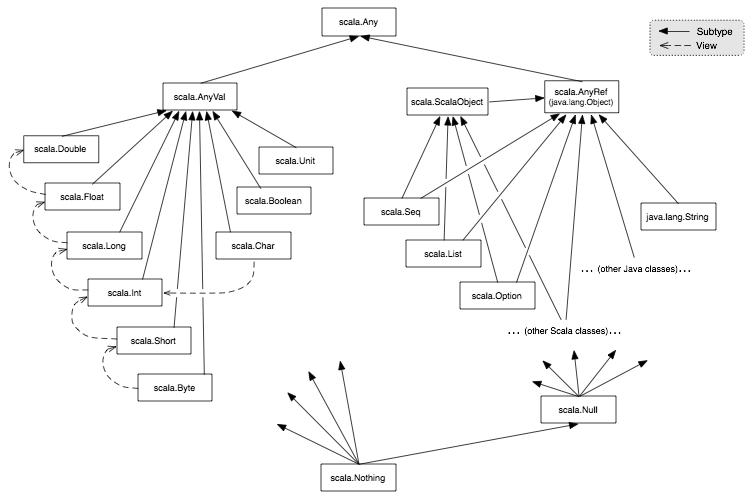
\includegraphics[width=\textwidth]{Bilder/classhierarchy}
  \caption{Vererbungshierarchie einiger Scala-Klassen \cite{UnbekannterAutor2013}}
  \label{fig:classhierarchy}
\end{figure}

Es gibt in Scala Konstrukte, die den selbst definierten Typen aus \ac{SL} sehr ähnlich sind. Das wird anschaulich am Beispiel von Option (siehe Listing \ref{lst:option-in-sl-scala}). Für sie kann die Übersetzung formalisiert werden. Mehr dazu im Abschnitt \ref{subsec:translate_type}. Es wurden aber auch andere Typen wie \lstinline!Seq[A]! übersetzt, deren innere Struktur sich stark von ihrem SL Äquivalent unterscheiden.

\begin{lstlisting}[caption=Option in SL und Scala, label=lst:option-in-sl-scala, float=h]
Option in SL:
PUBLIC DATA Option a = Some a | None

Option in Scala:
sealed abstract class Option[+A] ... { ... }

final case class Some[+A](x: A) extends Option[A] { ... }

case object None extends Option[Nothing] { ... }
\end{lstlisting}

\subsection{Funktion $translate_{type}$}
\label{subsec:translate_type}

%translate type formalisieren. möglich für option

Bei der Wahl eines SL-Partnertyps für einen Scala-Typ sollte auf zwei Bedingungen geachtet werden:

\begin{enumerate}
 \item{Die Typen sollten semantisch ähnlich sein.}
 \item{Es sollte eine semantisch sinnvolle, bijektive Abbildung zwischen den Werten der beiden Typen existieren. }
\end{enumerate}

Wie wir im Abschnitt \ref{sec:value-transformation} sehen werden, wird die zweite Bedingung für einige primitive Datentypen von Scala verletzt. Insbesondere für die ganzzahligen Primitiven kann sie nicht eingehalten werden. Da dadurch eine entsprechende Fehlerbehandlung unumgänglich wurde und um die Bedienung zu erleichtern, wurden alle Fließkommaprimitiven von Scala mit \lstinline!Real! und die ganzzahligen Primitiven mit \lstinline!Int! assoziiert.

\begin{table}[h]
\caption{Die Funktion $translate_{type}$}
\centering
\begin{tabular}{l|llllllllllllll}
\multicolumn{2}{l}{Primitive Datentypen:}\\
Scala-Typ & Byte & Float & Char & String & Boolean & Unit \\
 & Short & Double\\
 & Int\\
 & Long\\
SL-Typ & Int & Real & Char & String & Bool & Void \\
\addlinespace
\multicolumn{2}{l}{Andere:} \\
Scala-Typ & Seq[A] & Tuple2[A,B] & Option[A] & Either[A,B] \\
SL-Typ &  List a & Pair a b & Option a & Either a b \\
\end{tabular}
\label{tab:translate_type}
\end{table}


Bei generischen Datentypen wie \lstinline!Seq[A]! folgt aus den oben genannten Bedingungen, dass die Anzahl der Typparameter der Partnertypen gleich sein sollte. Wenn ein generischer Datentyp übersetzt werden soll, wird versucht die Typparameter rekursiv zu übersetzen. Ist dies möglich, kann auch der gesamte Typ übersetzt werden. Also würde \lstinline!Seq[Option[Long]]! zu \lstinline!List Option Int! übersetzt werden. Eine vollständige Auflistung von $translate_{type}$ findet sich in Tabelle \ref{tab:translate_type}.

\subsection{Formalisierung von $translate_{type}$}
\label{subsec:formal-translate-typ}

Bei primitiven Datentypen in Scala wurden die SL-Äquivalente durch ihre semantische Gleichheit vorgegeben (siehe Tabelle \ref{tab:translate_type}). 

Für bestimmte Typ-Konstrukte aus Scala kann die Übersetzung formalisiert werden. Sei dafür $Model$ durch folgende Grammatik beschrieben:

\begin{tabular}{lll}
\emph{Model} & ::= & \emph{Base} ; \emph{$Sub^+$}\\
\emph{Param} & ::= & \textbf{[ $\mathbf{V_1, \dots ,V_n}$ ]}\\
\emph{Base}  & ::= & \textbf{sealed abstract class} \emph{BaseName Param}\\
\emph{Sub}   & ::=   & \textbf{final case class} \emph{TypeName Param} \textbf{(} $Field^+$ \textbf{) extends} \emph{BaseName Param}\\
 & | & \textbf{case object} \emph{TypeName} \textbf{extends} \emph{BaseName} \textbf{[ Nothing$\,,\dots,\,$Nothing ]}\\
\emph{Field} & ::= & \emph{Name} \textbf{:} \emph{TypeName}\\
\\
\end{tabular}

Dabei sei $BaseName$ ein fester lokaler Typname, also alle Definitionen von $Sub$ erben von der gleichen abstrakten Klasse, $TypeName$ und $Name$ sind gültige Scala-Bezeichner. Damit wir diese Art von Klassen in einen SL-Typ übersetzen können, müssen alle Typvariablen, die in den $Sub$ Definitionen benutzt werden, bereits in der $Base$-Klasse definiert werden. Also $Param$ ist konstant für jede Instanz von $Model$.

Dann kann $translate_{type}$ folgendermaßen definiert werden, wobei = durch $\hat{=}$ ersetzt wird, da es in SL Teil der Syntax ist:

\begin{centering}
$translate_{type}(Model)\:\hat{=}$\\
\textbf{DATA} $t_{Name}(BaseName)\:t_{Param}(Param)$ \textbf{=} $t_{Case}(Sub_1)$ \textbf{|} $\dots$ \textbf{|} $t_{Case}(Sub_n)$\\
\end{centering}

mit:

\begin{equation*}
t_{Param}( \textbf{[ } \mathbf{V_1, \dots, V_n} \textbf{ ]} )\:\hat{=}\: t_{TypVar}(\mathbf{V_1} ) \dots t_{TypVar}(\mathbf{V_n} )
\end{equation*}
\begin{gather*}
t_{Case}(\textbf{final case class }TypeName \: Param\:\textbf{(}\mathbf{N_1:T_1, \dots, N_n:T_n}\textbf{)} \textbf{ extends }\dots )\:\hat{=}\\t_{Name}(TypeName)\:t_{Type}(T_1) \dots t_{Type}(T_n)\\
t_{Case}(\textbf{case object } TypeName\textbf{ extends }BaseName\textbf{ [ Nothing}\, ,\dots,\,\textbf{Nothing ]})\:\hat{=}\\
t_{Name}(TypeName)
\end{gather*}
und
\begin{equation*}
t_{Type}(x)\:\hat{=} \begin{cases}
        t_{TypeVar}(x)  &|\, x \in \{V_1, \dots , V_n\}\\
        translate_{type}(x) &|\, \text{sonst}
        \end{cases}
\end{equation*}

Wobei $t_{Name}$ einem Scala-Bezeichner einen SL-konformen Bezeichner  und $t_{TypeVar}$ einer Typvariable eine eindeutige SL-konforme Typvariable zuordnet. Eine komplette Übersetztung ist nur möglich, wenn $t_{Type}$ jedes $T_x$ übersetzen kann.

Dieses Schema wurde von einem Schema zum Übersetzen von \textbf{sealed trait}s im Paper von Höger et al.\cite{Hoger2013} inspiriert. Mit Hilfe dieser Schemata können einige der Scala-Typen in SL-Typen übersetzt werden. Wie man im Listing \ref{lst:option-in-sl-scala} sehen kann, folgt die Definition von \lstinline!Option[A]! dem hier vorgestellten Schema. Die Definition von \lstinline!Option a! ist eine mögliche Lösung des Aufrufs von $translate_{type}$. Ein weiterer übersetzbarer Typ ist \lstinline!Either[A]!.

Im Rahmen dieser Arbeit wurden alle Übersetzungen händisch programmiert, da Typen der Standardbibliotheken von Scala und SL miteinander assoziiert wurden\footnote{Es wurden also keine Typen für SL zu Scala-Typen generiert. Da Klassenmethoden im Moment nicht automatisch übersetzt werden können, hätte man keine Funktionen, die auf den generierten Typen operieren.}. Es wurde sich aber bei einigen Typen an dem hier beschriebenen Schema orientiert. Bei anderen wie \lstinline!Seq[A]! war dies nicht möglich, da sich die innere Struktur von seinem SL-Äquivalent zu sehr unterscheidet.


\section{Darstellungsübersetzung}
\label{sec:value-transformation}

In diesem Abschnitt wird beschrieben, wie Scala-Werte in SL-Werte bzw. zurück übersetzt werden. 

Grundsätzlich gelten drei Annahmen: 
\begin{enumerate}
 \item Die Wertübersetzungsfunktionen werden anhand des Scala-Typs gewählt.
 \item Werte werden von Scala nach SL und umgekehrt übersetzt.
 \item Die Wertübersetzungsfunktionen sind in Scala implementiert. Das heißt, wir können die Darstellung der Scala-Werte im JRE ignorieren, müssen aber die JS-Darstellung der SL-Werte verstehen.
\end{enumerate}

Zunächst wird die Übersetzung von primitiven Werten behandelt. Später werden komplexere Werte übersetzt.

\subsection{Übersetzung von primitiven Werten}
\label{subsec:primitive-value-translation}

\begin{savenotes}
\begin{table}[h]
\caption{Wertebereich der primitiven Datentypen in Scala und SL\cite[S. 28-30]{Ecma2011}\cite{Oracle2011}}
\centering
\begin{tabular}{lll}
SL-Typ & JS-Darstellung und Wertebereich & Scala-Typ und Wertebereich \\
\midrule
Int    & Number $[-2^{53} + 1, 2^{53} -1]$\footnote{Alle Zahlendatentypen werden in \ac{JS} durch den primitiven Number-Datentyp dargestellt. Dies ist eine Gleitkommazahldarstellung nach dem IEEE 754 Standard mit einer Breite von 64 Bit. In dieser Darstellung können Ganzzahlwerte von $-2^{53} + 1$ bis $2^{53} -1$ korrekt dargestellt werde.}    &  Byte  $[-128, 127]$\\
Int    & Number $[-2^{53} + 1, 2^{53} -1]$ & Short $[-2^{15}, 2^{15}-1]$\\
Int    & Number $[-2^{53} + 1, 2^{53} -1]$ & Int   $[-2^{31}, 2^{31}-1]$\\
Int    & Number $[-2^{53} + 1, 2^{53} -1]$ & Long  $[-2^{63}, 2^{63}-1]$\\
\addlinespace
Real   & Number (IEEE 754 64-Bit)          & Float  (IEEE 754 32-Bit)\\
Real   & Number (IEEE 754 64-Bit)          & Double (IEEE 754 64-Bit)\\
\addlinespace
Bool   & Boolean ${true, false}$           & Boolean ${true, false}$\\
\addlinespace
Char   & String (Länge 1) (16-Bit)         & Char (16-Bit)\\
\addlinespace
String& String\footnote{Die maximale Länge von Strings in \ac{JS} und Scala ist implementationsabhängig.} (maximale Länge: ?)    &  String (maximale Länge: ?)\\
\end{tabular}
\label{tab:primitives-borders}
\end{table}
\end{savenotes}

Vor allem bei der Übersetzung von Primitiven existiert das Problem der unterschiedlichen Wertebereiche. Man kann zwar jeden Wert des Scala-Typs \lstinline!Byte! in einen Wert des SL-Typs \lstinline!Int! übersetzen, aber nicht umgekehrt. In der Tabelle \ref{tab:primitives-borders} werden die Wertebereiche für primitive Typen aufgelistet. Kann ein Wert von einer Darstellungsform nicht in die andere Darstellungsform umgewandelt werden, muss dieser Fehler behandelt werden (siehe Abschnitt \ref{subsec:example-option-translator}). Insbesondere bei den ganzzahligen Primitiven ist das Problem unumgänglich.  Für ihre Wertebereiche gilt:

\begin{center}
$|$\lstinline!Scala Int!$| < |$\lstinline!Number bzw. SL Int!$| < |$\lstinline!Scala Long!$|$
\end{center}

\subsection{Übersetzung von komplexen Werten}

Bei nicht primitiven Werten ist mehr Aufwand nötig. Dafür müssen wir zunächst die JS-Darstellung von selbst definierten SL-Typen verstehen\footnote{Das beschriebene Schema wurde aus dem SL-Compiler generierten Code abgeleitet. Es ist nicht dokumentiert.}.

\begin{lstlisting}[caption=Beispiel eines selbst definierten Typs, label=lst:example-datatype-sl]
DATA People a b = Alice | Bob Int | Cesar a b | Octavian
\end{lstlisting}

Die einzelnen Konstruktoren erhalten entsprechend ihrer Reihenfolge eine Konstruktor-ID (\lstinline!_cid!) beginnend bei $0$. Hat ein Konstruktor keine Parameter, wird er nur durch seine \lstinline!_cid! dargestellt. Andernfalls wird ein Objekt erzeugt. Dies besitzt das Attribut \lstinline!_cid! sowie entsprechend der Anzahl der Parameter Attribute, die von \lstinline!_var0! bis \lstinline!_varN! benannt sind. Die JS Darstellung von dem Beispieltyp aus Listing \ref{lst:example-datatype-sl} findet sich in der Tabelle \ref{tab:js-code-of-people}.

\begin{table}[h]
\caption{JS-Darstellung des SL-Typen \lstinline!People Char Bool!}
\centering
\begin{tabular}{ll}
 \ac{SL}              &  \ac{JS} Darstellung \\
\lstinline!Alice!           &  \lstinline!0! \\
\lstinline!Bob 42!          &  \lstinline!{ "_cid" => 1, "_var0" => 42 }! \\
\lstinline!Cesar "a" true!  &  \lstinline!{ "_cid" => 2, "_var0" => "a", "_var1" => true }! \\
\lstinline!Octavian!        &  \lstinline!3! \\
\end{tabular}
\label{tab:js-code-of-people}
\end{table}

Mit Hilfe dieser Informationen und dem Schema aus Absatz \ref{subsec:formal-translate-typ} können jetzt Option-Werte zwischen SL und Scala ausgetauscht werden. In der Tabelle \ref{lst:option-in-sl-scala} wurden beispielhaft einige Werte vom Typ \lstinline!Option[Int]! übersetzt. In Abschnitt \ref{subsec:example-option-translator} wird auf die Implementation der Übersetzung von \lstinline!Option[A]! noch einmal genauer eingegangen.

\begin{table}[h]
\caption{Übersetzung von \lstinline!Option! Werten}
\centering
\begin{tabular}{lll}
Scala                   & JS-Darstellung                        & SL \\
\midrule
\lstinline!Option[Int]! &                                            & \lstinline!Option Int! \\
\lstinline!Some(15)!    & \lstinline!{ "_cid" => 0, "_var0" => 15 }! & \lstinline!Some(15)! \\
\lstinline!None!        & \lstinline!1!                              & \lstinline!None! \\
\end{tabular}
\end{table}

Wie bereits im Abschnitt \ref{subsec:formal-translate-typ} erwähnt, ist es auch möglich ohne das dort beschriebene Schema Werte zu übersetzen. Betrachten wir dies am Beispiel \lstinline!Seq[A]!. \lstinline!Seq[A]! ist ein Scala-Trait, der ein Interface zum Arbeiten auf verketteten Listen darstellt. Er kann mit \lstinline!val a: Seq[Int] = Seq(1,2,3)! in­s­tan­zi­ie­rt werden. In den meisten Fällen wird \lstinline!Seq[A]! intern als \lstinline!List[A]! dargestellt, muss es aber nicht. Die innere Struktur ist unbekannt, aber man kann mit Hilfe von Methode oder pattern matching auf die Elemente der Liste zugreifen. 

Das SL-Äquivalent \lstinline!List a! hat folgende Typdefinition:

\begin{center}
\lstinline!DATA List a = Nil | Cons a (List a)!
\end{center}

Mit pattern matching, rekursiven Funktionen und dem Wissen über die JS-Darstellung von \lstinline!List a!, ist es trotzdem möglich solche Werte zu übersetzen. In der Tabelle \ref{tab:seq-int} wurden einige Werte beispielhaft übersetzt.

\lstset{basicstyle=\ttfamily\small, numbers=none}
\begin{table}[h]
\caption{Übersetzung von \lstinline!Seq[Int]!-Werten}
\centering
\begin{tabular}{lll}
Scala                & JS-Darstellung                        & SL \\
\midrule
\lstinline!Seq()!    & \lstinline!0! & \lstinline!Nil! \\
\lstinline!Seq(1)!   & \lstinline!{ "_cid" => 1, "_var0" => 1, "_var1" => 0 }!                              & \lstinline!Cons 1 Nil! \\
\lstinline!Seq(3,4)! & 
\begin{lstlisting}
{ "_cid" => 1
, "_var0" => 3
, "_var1" => 
  { "_cid" => 1
  , "_var0" => 4
  , "_var1" => 0
  }
}
\end{lstlisting} & \lstinline!Cons 3 (Cons 4 Nil)! \\
\end{tabular}
\label{tab:seq-int}
\end{table}
% reset lst settings
\lstset{basicstyle=\ttfamily\small, numbers=left, numberstyle=\tiny}

Die Übersetzung von anonymen Funktionen, also Werten die eine Funktion darstellen, ist im Moment nicht möglich, da kein adäquater Weg gefunden wurde, um ihre Darstellung zwischen Scala und JS auszutauschen.

\section{Erläuterung der Implementation}
\label{sec:trans-implementation}

In der momentanen Implementation wird $translate_{type}$ durch \lstinline!Seq[AbstractTranslator]! dargestellt. Dadurch ist es möglich auch Teilmengen von $translate_{type}$ zu benutzen. Dabei stellt eine Klasse, die von \lstinline!AbstractTranslator! erbt, ein Paar zwischen einem Scala-Typ und einem SL-Typ dar. Die Klasse ist nach dem jeweiligen Scala-Typen, den sie übersetzt, benannt. Zum Beispiel stellt die Klasse \lstinline!SeqTranslator! die Verbindung zwischen dem Scala-Typ \lstinline!Seq[A]! und dem SL-Typ \lstinline!List a! her. 

Die Hauptmethode von \lstinline!AbstractTranslator! ist \lstinline!translate! (siehe Listing \ref{lst:main-function-translate}). Ihr wird ein Scala-Typ übergeben. Wenn der übergebene Scala-Typ der Klasse entspricht, erhält man als Rückgabewert den entsprechenden SL-Typen, die Import Statements, um die entsprechenden SL-Module zu laden\footnote{Bei primitiven SL-Typen sind diese leer. Für den SL-Typ \lstinline!List.List Opt.Option Int! würde \lstinline!IMPORT "std/option" AS Opt, IMPORT "std/list" AS List! zurück gegeben werden.} sowie die \ac{AST}-Repräsentation der Wertübersetzungsfunktionen von Scala nach SL und umgekehrt. Andernfalls wird \lstinline!None! zurückgegeben.

\begin{lstlisting}[caption=Hauptfunktion in AbstractTranslator, label=lst:main-function-translate]
def translate
  ( context: MacroCtxt )
  ( input: context.universe.Type, translators: Seq[AbstractTranslator] )
: Option[( String, 
           Set[String], 
           context.Expr[Any => JValue], 
           context.Expr[JValue => Any] )]
\end{lstlisting}

Weitere Parameter sind \lstinline!context! und \lstinline!translators!. \lstinline!context! ist der Makro Kontext\footnote{siehe Kapitel \ref{chap:scala-compiler-macros}}. Er wird benötigt, um \ac{AST}s aufzubauen und den übergebenen Typen zu prüfen. Mit \lstinline!translators! wird der Teil von $translate_{type}$ übergeben, mit dem Spezialisierungen eines generischen Typs übersetzt werden können.

Möchte man einen Scala-Typ nicht nur gegen eine Klasse prüfen, kann man die Hilfsfunktion \lstinline!useTranslators! aus dem companion object von \lstinline!AbstractTranslator! nutzen.

\begin{lstlisting}[caption=Statische Hilfsfunktion in AbstractTranslator, label=lst:hilfsfunktionen]
def useTranslators
  ( context: MacroCtxt )
  ( input: context.universe.Type, translators: Seq[AbstractTranslator] )
: Option[( String,
           Set[String], 
           context.Expr[Any => JValue], 
           context.Expr[JValue => Any] )]
\end{lstlisting}

\lstinline!translators! gibt hier an, welche Teilmenge der Funktion $translate_{type}$ man nutzen möchte\footnote{\lstinline!translators! wird in diesem Fall auch für die Spezialisierungen von generischen Typen benutzt.}. 

Die Wertübersetzungsfunktionen haben die Signatur \lstinline!Any => JValue! bzw. \lstinline!JValue => Any!. \lstinline!JValue! ist Teil der json4s Bibliothek \cite{Json4s}, die benutzt wird, um JS-Werte zu erzeugen. Insbesondere übernimmt sie in der aktuellen Implementation die Übersetzung der primitiven Werte.

\subsection{OptionTranslator als Beispiel}
\label{subsec:example-option-translator}

Der \lstinline!OptionTranslator! bildet die Verbindung zwischen dem Scala-Typ \lstinline!Option[A]! und seinem SL-Pendant \lstinline!Option a! ab. 

Wie bereits erwähnt, ist die Hauptfunktion \lstinline!translate! (siehe Listing \ref{lst:main-function-translate}). In ihr wird zunächst mit reflection überprüft, ob der übergebene Typ (\lstinline!input!) ein Subtyp von \lstinline!Option[Any]! ist. Durch die Definition von \lstinline!Option[A]! (\lstinline!sealed! und \lstinline!final case! siehe Listing \ref{lst:option-in-sl-scala}) können wir uns sicher sein, dass übergebene Werte nur vom Typ \lstinline!Some[A]! oder \lstinline!None! sind. Wieder mit reflections wird der Typ der Spezialisierung \lstinline!A! bestimmt. Ist dieser Typ mit Hilfe der übergebenen Translator-Klassen (\lstinline!translators!) übersetzbar, wird das Ergebnis zusammengestellt. In jedem anderen Fall wird \lstinline!None! zurückgegeben.

Das Ergebnis besteht aus dem SL-Typ (zum Beispiel \lstinline!Option Int!), der Import-Anweisung (mindestens \lstinline!IMPORT "std/option" AS Opt!) und den ASTs der beiden Wertübersetzungsfunktionen. Die Wertübersetzungsfunktionen werden im companion object definiert, um sie besser mit Unit-Tests zu testen. Mit Hilfe der Funktion \lstinline!reify! aus der Makro API von Scala wird aus Scala-Code der entsprechende AST generiert. Grundsätzlich könnte der AST, der die Wertübersetzung repräsentiert, eine anonyme Funktion und kein Funktionsaufruf sein. In späteren Kapiteln heißen die Funktionen zum Übersetzen deshalb immer \lstinline!scala_to_js! und \lstinline!js_to_scala!.

\begin{lstlisting}
reify ( {
( i : Any ) = > OptionTranslator.scalaToJsOption ( i , expr_s2j )
} )
\end{lstlisting}

\lstinline!expr_s2j! ist in diesem Fall die Wertübersetzungsfunktion des Typs der Spezialisierung. 

\begin{lstlisting}
def scalaToJsOption( input: Any, f: Any => JValue ): JValue = {
  import org.json4s._
  input match {
    case Some( x ) => {
      val tmp: List[( String, JValue )] = 
        List( "_cid" -> JInt( 0 ), "_var0" -> f( x ) )
      JObject( tmp )
    }
    case None => JInt( 1 )
    case _ => throw new IllegalArgumentException
  }
}
\end{lstlisting}

Wird an die Wertübersetzungsfunktion ein unerwarteter Wert (oder bei primitiven Typen ein Wert außerhalb der zulässigen Grenzen) übergeben, wird eine \lstinline!IllegalArgumentException! erzeugt.

Möchte man einen neuen Scala-Typ übersetzen bzw. zu $translate_{type}$ hinzufügen, muss eine neue Translator-Klasse geschrieben werden. Eine entsprechende Anleitung findet sich im Anhang \ref{sec:new-translator-class}.

\chapter{Scala Compiler Makros}
\label{chap:scala-compiler-macros}

Im \ref{cha:sl-introduction}. Kapitel wurde SL vorgestellt. Eine strikt getypte, funktionale Sprache, die in JS-Code übersetzt wird.

SL brachte Höger et al. auf die Idee mit Hilfe von Scala Compiler Makros eine strikt getypte Abstraktion für JS in Scala einzubinden\cite{Hoger2013}. Um ihre Ergebnisse zu demonstrieren, haben sie eine Beispielwebanwendung mit Hilfe des Play-Frameworks\cite{Play1} geschrieben. 

Play ist ein \ac{MVC}-Framework für Webanwendungen, welches in Scala geschrieben ist. Play vereinfacht die Erstellung von strukturierten Webanwendungen. Auch innerhalb dieser Arbeit wird es genutzt, um die Einbettung von SL in Scala zu erproben.

Es konnte das Problem der dynamischen Typisierung von JS behoben werden, aber ein anderes blieb offen. Bis jetzt war es nicht möglich, SL- bzw. JS-Code abhängig von der Scala-Umgebung zu generieren. Insbesondere für Webanwendung stellt dies ein Problem dar. Es sollte möglich sein, den JS-Code zum Beispiel mit einem Benutzernamen zu personalisieren. 

Mit Hilfe der im Kapitel \ref{cha:model-sharing} beschriebenen Einbettung von Scala-Werten/-Typen in SL ist es jetzt möglich dieses Problem zu lösen.

Um den SL-Code von der Scala-Umgebung abhängig zu machen, wurden zwei Ansätze verfolgt. Zum einen ist es jetzt möglich, Scala-Werte direkt im SL-Code zu nutzen. Dazu werden Platzhalter in den SL-Code eingefügt, die dann durch übersetzte Scala-Werte ersetzt werden.

Zum anderen können Scala-Funktionen aus SL-Code heraus aufgerufen werden. Dazu wird aus einer Scala-Funktion eine SL-Funktion generiert, die die Scala-Funktion über asynchrone Kommunikation mit dem Server und Scala reflections aufruft.

Um diese Lösungen zu realisieren, wurden zwei Scala Compiler Makros geschrieben. Diese werden im Laufe dieses Kapitels vorgestellt.

\section{Makros und ihre Abhängigkeiten}
\label{sec:project-structure}

Um Scala Funktionen für die Verwendung in \ac{SL}-Code zu markieren, wurde die macro annotation \lstinline!sl_function! geschrieben, welche im Abschnitt \ref{sec:annotation-macro} behandelt wird. Im darauf folgenden Abschnitt \ref{sec:inline-macro} wird beschrieben, wie statischer \ac{SL} Code mit Hilfe des def macros \lstinline!slci! eingebunden wird und welche Veränderungen gemacht werden mussten, um Scala Werte und annotierte Funktionen benutzen zu können. Beide Makros binden den Trait \lstinline!MacroConfig! ein, in dem grundsätzliche Konfigurationen definiert sind. Zur Übersetzung der Typen und Werte werden die Translator-Klassen genutzt. Einen Überblick über das Projekt bietet die Abbildung \ref{fig:project-overview}.

\begin{figure}[h] 
  \centering
     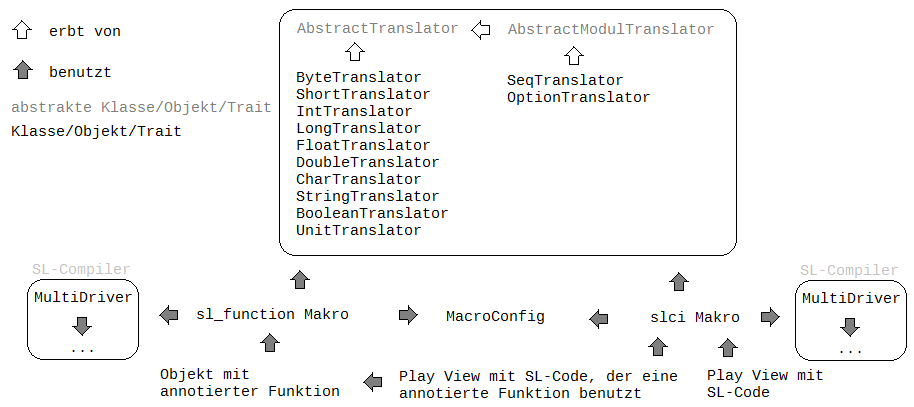
\includegraphics[width=\textwidth]{Bilder/projektstruktur}
  \caption{Projektübersicht}
  \label{fig:project-overview}
\end{figure}

\subsection{Konfiguration der Makros}
\label{subsec:macro-config}

Im Trait \lstinline!MacroConfig! werden die beiden hier programmierten Makros konfiguriert. In den anschließenden Abschnitten wird sich darauf bezogen. Die wichtigsten Konfigurationsparameter sind:

\begin{description}
 \item[assets\_dir] Gibt an, in welchem Ordner die SL-Quelldateien und ihre Kompilate liegen. Im Moment \lstinline!/projekt_ordner/public/sl/!.
 \item[inline\_sl\_macro\_folder] Gibt den Unterordner von \lstinline!assets_dir! an, in dem die SL-Module/-Quelldateien und ihre Kompilate liegen, die vom def marco slci generiert werden. Im Moment: \lstinline!generated_inline/!.
 \item[annotation\_sl\_macro\_folder] Gibt den Unterordner von \lstinline!assets_dir! an, in dem die SL-Module liegen, die von der macro annotation sl\_function generiert werden. Im Moment: \lstinline!generated_annotation/!.
 \item[inline\_sl\_macro\_handler\_uri] Gibt die URL an, unter welcher der Server auf asynchrone Kommunikation lauscht, um per reflection annotierte Scala-Funktionen aufzurufen. Im Moment ist dies die relative URL \lstinline!/ajax!.
\end{description}

Wird in der Konfiguration etwas geändert, muss das ganze Projekt neu kompiliert werden. Insbesondere müssen alle generierten SL-Module neu erstellt werden.

%TODO Probleme mit namen von scala funktionen

\section{Macro Annotation sl\_function }
\label{sec:annotation-macro}

Mit macro annotations kann in den Übersetzungsprozess von Scala eingegriffen werden\cite{EPFL1}. Es ist möglich den annotierten Code zu verändern\footnote{Es können Funktionen, Klassen, Objekte, Typparameter oder Funktionsparameter annotiert werden.}. Mit dem geschriebenen Makro können nur Funktionen annotiert werden. Für jede Funktion wird eine Hilfsfunktion und ein \ac{SL}-Modul erzeugt. Die Hilfsfunktion soll den Aufruf im Rahmen von Ajax-Anfragen erleichtern. Das \ac{SL}-Modul ermöglicht es, diesen Aufruf typsicher in \ac{SL}-Programme einzubinden. Beispielhaft wird das An­no­tie­ren einer Funktion anhand der im Listing \ref{lst:example-function} beschriebenen Funktion \lstinline!factorial! betrachtet.


\begin{lstlisting}[caption=Scala Beispielfunktion, label=lst:example-function, float=h]
-- Foo.scala
package example

object Foo {
  @sl_function def factorial( i: Int ): Long = {...}
}
\end{lstlisting}

\subsection{Anforderungen an eine Funktion}

Die zu übersetzende Funktion muss gewisse Anforderungen erfüllen. Wenn wir sie im Rahmen von Ajax-Anfragen benutzen wollen, muss sie statisch aufrufbar sein, also:
\begin{itemize}
  \item[-]{Sie muss in einem Objekt definiert sein.}
  \item[-]{Ihre Signatur darf keine Typparameter enthalten.}
  \item[-]{Die Funktion darf nicht als \lstinline!private! oder \lstinline!protected! markiert sein.}
 \end{itemize}

Andere Anforderungen ergeben sich aus der Implementation bzw. wurden aufgestellt, um die Implementation zu erleichtern:

\begin{description}
 \item[Die Ein- und Ausgangstypen müssen sich in SL-Typen übersetzen lassen.]{Gilt dies nicht, kann keine passende SL-Funktion erzeugt werden.}
 \item[Die Funktion muss einen Rückgabetyp definieren.]{Andernfalls müsste der Rückgabetyp erst über reflection bestimmt werden. Der Scala Compiler kann den Rückgabetyp wahrscheinlich bestimmen, dies wurde aber nicht in Angriff genommen.}
 \item[Die Funktion darf nur eine Parameterliste haben.]{Mehrere Parameterlisten könnten in eine zusammengefasst werden. Da diese Einschränkung aber nur minimal ist und es den Aufruf der Funktion über reflection erschwert hätte, wurde davon Abstand genommen.}
 \item[Standardwerte von Parametern werden ignoriert.]{In der aktuellen Implementation werden die Standardwerte eines Parameters ignoriert. Eine entsprechende Compilerwarnung wird erzeugt.}
 \item[Der Funktionsname darf keine ungewöhnlichen Zeichen enthalten.]{Da sich der Name der Funktion im Namen und Pfad des erzeugten Moduls widerspiegelt, sind nur die Zahlen von 0 bis 9 sowie kleine Buchstaben von a bis z erlaubt. Ähnliche Einschränkungen gelten für die übergeordneten Pakete sowie den Namen des Objekts in dem die Funktion definiert ist.}
\end{description}

\subsection{SL-Modul}
\label{subsec:sl-modul}

Für jede annotierte Funktion wird ein Modul erstellt. Dass heißt eine SL-Quelldatei erstellt, die den entsprechenden SL-Code enthält.

Das Modul enthält zwei Funktionen, jeweils für den asynchronen und synchronen Aufruf der Scala-Funktion über Ajax. Das Ergebnis wird in \lstinline!Option! gekapselt, um auf Fehler in der Kommunikation mit dem Server reagieren zu können. Im Fehlerfall wird \lstinline!None! zurückgegeben. Das Erzeugen der Ajax-Anfrage und das Behandeln des Ergebnisses passiert in den \ac{JS}-Funktionen \lstinline!_sendRequestSync()! und \lstinline!sendRequestAsync()!. Diese Funktionen sind in der \ac{JS}-Bibliothek std/\_scalafun.js definiert. 

Weiterhin enthält das Modul in Kommentaren den Namen der aufgerufenen Funktion sowie den voll qualifizierten Namen des Objektes in dem die Funktion definiert ist. Diese Informationen werden gebraucht, um Abhängigkeiten zwischen der Scala Funktion und ihrer Benutzung in \ac{SL}-Code aufzulösen. Genauer wird dies im Abschnitt \ref{subsec:use-scala-function-in-sl} beschrieben. Das Modul wird direkt nach dem Erstellen kompiliert.

Zu erwähnen sind noch die Import-Anweisungen. Die Quelldateien \lstinline!std/option! und \lstinline!std/_scalafun! werden immer importiert, da sie offensichtlich immer gebraucht werden. Enthält aber die Funktionsdefinition der annotierten Funktion einen Scala-Typ, dessen SL-Pendant in einem externen Modul definiert ist (zum Beispiel \lstinline!List a!), muss dieses auch importiert werden. Eine entsprechende Import-Anweisung wird dann hinzugefügt.

\begin{lstlisting}[caption=SL-Modul factorial.sl zur Funktion aus Listing \ref{lst:example-function}, label=lst:example-sl-modul, float=h]
-- DO NOT ALTER THIS FILE! --------------------------------
-- cp: example.Foo
-- fn: factorial
-- --------------------------------------------------------
-- this file was generated by @sl_function macro ----------
-- on 20-06-2014 ------------------------------------------
IMPORT EXTERN "std/_scalafun"
IMPORT "std/option" AS Opt

-- this functions should call the scala function:
-- example.Foo.factorial
PUBLIC FUN factorialSync : Int ->  DOM ( Opt.Option (Int) )
DEF factorialSync p0 = {| _sendRequestSync( ... ) ($p0) |}  : DOM ( Opt.Option (Int) )

PUBLIC FUN factorialAsync : ( Opt.Option (Int) -> DOM Void )  -> Int -> DOM Void
DEF factorialAsync callbackFun p0 = {| _sendRequestAsync( ... )  ($callbackFun, $p0) |} : DOM Void
\end{lstlisting}

\subsection{Hilfsfunktion}
\label{subsec:helperfunction}

Um den Aufruf mit Ajax-Anfragen zu erleichtern, wird eine Hilfsfunktion definiert. Sie kapselt die eigentliche Scala-Funktion. Sie erhält die Parameter als \lstinline!JValue!. Die Parameter werden mit Hilfe der Funktionen aus den Translator Klassen in Scala Werte übertragen und dann auf den passenden Typ gecasted. Anschließend wird mit ihnen die eigentlich Funktion aufgerufen. Das Ergebnis wird in ein \lstinline!JValue! Wert umgewandelt und zurückgegeben.

Die Funktionen \lstinline!scala_to_sl! und \lstinline!sl_to_scala! sind nur Platzhalter. Wie diese Funktionen genau definiert sind, hängt von der Implementation der entsprechenden Translator-Klasse ab (siehe Abschnitt \ref{subsec:example-option-translator}).

\begin{lstlisting}[caption=Hilfsfunktion zur Funktion aus Listing \ref{lst:example-function}, label=lst:helperfunction, float=h]
-- Foo.scala
package example

object Foo {
  @sl_function def factorial( i: Int ): Long = {...}
  
  def factorial_sl_helper( p1: org.json4s.JValue ) : org.json4s.JValue = {
    scala_to_sl(factorial(sl_to_scala(p1)))
  }
}
\end{lstlisting}

\subsection{Ablauf eines sl\_function Aufrufs}

Wie bereits erwähnt, wird das Makro während der Übersetzung des Scala Programms aufgerufen. Der Aufruf des \lstinline!sl_function!-Makros folgt den letzten drei Abschnitten. Zunächst wird überprüft, ob die annotierte Funktion den Anforderungen genügt. Dann wird das Modul im Ordner \lstinline!annotation_sl_macro_folder! (siehe Abschnitt \ref{subsec:macro-config}) erzeugt und übersetzt.

Daraufhin wird der \ac{AST} der Hilfsfunktion erzeugt und diese hinter der annotierten Funktion in das Objekt eingefügt. 

Sollte es in einem der Schritte zu einem Fehler kommen, wird ein Compilerfehler erzeugt und die Übersetzung des Scala-Programms abgebrochen.

\subsection{Aufruf einer annotierten Funktion}
\label{subs:call-scala-functions}

Betrachten wir nun den Aufrufprozess einer Funktion im Ganzen am Beispiel der Funktion \lstinline!factorialSync! aus dem Listing \ref{lst:example-sl-modul}. Folgende Schritte werden durchlaufen:
\begin{enumerate}
 \item{Aufruf der Funktion \lstinline!factorialSync 5! im \ac{SL}-Code}
 \item{Aufruf der \ac{JS}-Funktion \lstinline!(_sendRequstSync( "\ajax", "example.Foo", "factorial" )) (5)!. Es werden der URL des Ajax-Handlers, der voll qualifizierte Name des Objekts und der Funktionsname übergeben. In einem zweiten Schritt wird der eigentliche Parameter (\ac{SL}-Codiert) übergeben.}
 \item{Die \ac{SL}-Parameter werden mit Hilfe der Bibliothek json.js \cite{Crockford2010} in einen JSON String umgewandelt und mit Funktions- und Objektname als Anfrage an die Adresse des Ajax-Handlers geschickt (siehe Tabelle \ref{tab:post-parameter}).}
 \item{Der Ajax-Handler wandelt die Funktionsparameter (\lstinline!5!) in \lstinline!JValue! Werte um \cite{Json4s} und ruft dann über reflection die Hilfsfunktion \lstinline!factorial_sl_helper! auf. Das Ergebnis (\lstinline!120!) des Aufrufs wird als JSON String zurück an den Client gesendet.}
 \item{Ist die Anfrage an den Server erfolgreich, wird \lstinline!Some(120)! zurückgegeben, andernfalls \lstinline!None!.}
\end{enumerate}

\begin{table}[h]
\caption{Post Parameter der Ajax-Anfrage}
\centering
\begin{tabular}{ll}
Parametername        &   Inhalt \\
\hline
object\_name   & Voll qualifizierter Name des Objekts \\
function\_name & Name der Funktion\\
params         & JSON encodierte Liste der übergebenen Parameter\\
\end{tabular}
\label{tab:post-parameter}
\end{table}

\section{Def Macro slci}
\label{sec:inline-macro}

Bis jetzt kann man nur Funktionen markieren. Nun soll \ac{SL} benutzt werden, um \ac{JS}-Code zu generieren und ihn auf Benutzerseite zu verwenden. Dazu wurde das \lstinline!slci!-Makro neu geschrieben und erweitert. Im Laufe der nächsten Abschnitte vollziehen wir die Entwicklungsschritte des Makros nach.

Mit def macros kann während des Übersetzungsprozesses von Scala in den Code eingegriffen werden \cite{EPFL2}. Der Aufruf solch eines Makros verhält sich wie eine Funktion, nur dass das Makro die \ac{AST}s der Parameter übergeben bekommt und einen \ac{AST} liefert, der den Aufruf des Makros ersetzt. Listing \ref{lst:slci-example} enthält einen beispielhaften Aufruf des slci-Makros.

\begin{lstlisting}[caption={Beispielaufruf des slci-Makros in einer Play-View}, label=lst:slci-example, float=h]
-- Example.scala.html
...
<script type="text/javascript">@{
Html(slci(
"""
PUBLIC FUN main : DOM Void
DEF main = ...
"""
))}
</script>
...
\end{lstlisting}

\subsection{Statischen SL-Code übersetzen}
\label{subsec:compile-static-sl}

Mit der Entwicklung eines Modulsystems für \ac{SL} musste das Einbetten von statischem Code neu geschrieben werden \cite{Bisping2013}. Die erste Version des \lstinline!slci!-Makros nutzte eine Version von \ac{SL} die \ac{JS}-Code erzeugt. Im Laufe des Studentenprojekts wurde davon Abstand genommen. Das Ergebnis der Übersetzung sind \ac{JS}-Dateien, die mit Hilfe von require.js\footnote{require.js ist eine JS-Bibliothek mit der JS-Dateien und -Module geladen werden können. Es ist besonders für die Benutzung in Browsern optimiert.} in Webseiten eingebettet werden \cite{RequireJS1}.

Entsprechend wird jetzt vom \lstinline!slci! Makro ein \ac{SL}-Modul erzeugt. Die Datei wird entsprechend des Ortes benannt, an dem \lstinline!slci! aufgerufen wird:
\begin{center}
\lstinline!<Dateiname>.<Zeilennummer>.sl!
\end{center}
Wenn diese Datei übersetzt werden kann, wird der Aufruf des slci-Makros durch einen String ersetzt. Der String repräsentiert ein JS-Snippet, das mit Hilfe von require.js das übersetzte Modul einbindet und seine \lstinline!main!-Funktion aufruft.

Neben require.js müssen noch andere \ac{JS}-Bibliotheken geladen werden. Möchte man \ac{SL}-Code in einer Webseite benutzen, müssen alle Bibliotheken eingebunden werden, die in Tabelle \ref{tab:js-libraries} aufgelistet sind.

\begin{table}[h]
\caption{Benötigte JS-Bibliotheken}
\centering
\begin{tabular}{ll}
jquery-1.9.0.min.js & Erleichtert Ajax-Anfragen. Wird vom sl\_function-Markro benötigt\cite{JQuery1}.\\
sl\_init.js         & Initialisiert die globale Variable \lstinline!sl! und konfiguriert require.js. \\
                    & Muss vor require.js geladen werden.\\
require.js          & Wird benötigt um SL-Module nachzuladen\cite{RequireJS1}.\\
json.js             & Zum Umwandeln von JS-Werten in ihre JSON-Repräsentation \\
                    & und zurück. Siehe Abschnitt \ref{subs:call-scala-functions}\cite{Crockford2010}.\\
\end{tabular}
\label{tab:js-libraries}
\end{table}

\subsection{Scala Variablen in SL nutzen}

Als Nächstes wurde die Verwendung von Scala-Variablen in \ac{SL}-Code implementiert. Anhand des Beispiels im Listing \ref{lst:slci-example-var} werden die dafür nötigen Schritte erklärt.

\begin{lstlisting}[caption={Beispielaufruf des slci-Macros mit Scala Variablen}, label=lst:slci-example-var, float=h]
slci(
"""
IMPORT "std/option" AS Option 
...
FUN foo : Option.Option Int
DEF foo = #s
...
""",
Some(3)
)
\end{lstlisting}

Die zu ersetzende Stelle wird durch einen Platzhalter (\lstinline!#s!) markiert. Der $n+1$-te Parameter von \lstinline!slci! wird dem $n$-ten Platzhalter zugeordnet. Falls die Anzahl der Parameter ungleich der Anzahl der Platzhalter ist, werden Compiler-Warnungen erzeugt oder die Übersetzung mit einem Fehler abgebrochen. 

Daraufhin werden die \lstinline!IMPORT!-Anweisungen analysiert und die entsprechenden Translator-Klassen geladen\footnote{Translator-Klassen, die in Standardtypen von SL übersetzen, werden immer geladen. Für \lstinline!IMPORT "std/option" AS Modulalias! würde die Instanz \lstinline!new OptionTranslator("Modulalias")! erzeugt werden.}.  Die von der Makro-API bestimmten Typen\footnote{Manchmal muss man den Typ annotieren. Das Literal \lstinline!5! hat den Typ \lstinline!Int(5)! und nicht \lstinline!Int!. Man schreibt also \lstinline!5:Int!.} der Parameter werden dann mit den zur Verfügung stehenden Translator-Klassen übersetzt.

Wenn alle Typen übersetzt werden konnten, werden die Platzhalter durch \ac{JS}-quotings ersetzt, die auf globale Variablen zugreifen. Im Beispiel aus Listing \ref{lst:slci-example-var} würde \lstinline!#s! durch \\*\lstinline!{| sl['5a40c735438fd9e1fd43657bd7f8564scalaParam1'] |} : Option.Option Int!\footnote{Der Name der JS-Variable folgt folgendem Schema: \\*\lstinline!<Hash des Macrokontexts>scalaParam<Parameternummer>!.} ersetzt werden. Der so erzeugte SL-Code wird dann, wie im Abschnitt \ref{subsec:compile-static-sl} beschrieben, übersetzt. 
Listing \ref{lst:slci-example-var-scala-code} enthält den vom Makro erzeugt Scala-Code. 

\begin{lstlisting}[caption={Erzeugter Scala-Code zum Listing \ref{lst:slci-example-var}}, label=lst:slci-example-var-scala-code, float=h]
{ 
"""
require(...);
// transformed scala variables    
sl['5a40c735438fd9e1fd43657bd7f8564scalaParam1'] = %s;
""".format( compact( render( scala_to_sl( Some(3) ) ) ) )
}
\end{lstlisting}

Mit den von den Translator-Klassen erzeugten Übersetzungsfunktionen, werden die Parameter in \ac{SL}-Werte übersetzt. Da sie zuerst als \lstinline!JValue!-Objekte vorliegen, müssen sie noch in \ac{JS}-Code überführt werden. Im Listing \ref{lst:slci-example-var-js-code} findet sich der nach einem Aufruf der Webseite erzeugte \ac{JS}-Code.

\begin{lstlisting}[caption={JS-Code zum Listing \ref{lst:slci-example-var}}, label=lst:slci-example-var-js-code, float=h]
require( 
  [ "generated_inline/example.template.scala.48.sl" ],
  function (tmp) { sl['koch.template.scala.1'] = tmp; }
);
// transformed scala variables 
sl['5a40c735438fd9e1fd43657bd7f8564scalaParam1'] = {"_cid":0,"_var0":3};
\end{lstlisting}

\subsection{Scala Funktionen in SL nutzen}
\label{subsec:use-scala-function-in-sl}

Im Abschnitt \ref{sec:annotation-macro} wurde erklärt, wie Scala-Funktionen für die Verwendung in \ac{SL}-Code markiert werden. Für die markierten Funktionen werden \ac{SL}-Module erzeugt. Wenn ein solches Modul geladen wird\footnote{Der Pfad des Moduls fängt in der aktuellen Konfiguration mit \lstinline!generated_annotation/! an.}, werden am Anfang des vom Makro erzeugten Scala-Codes \lstinline!import!-Anweisungen eingefügt, die auf die referenzierten Scala Funktionen verweisen. Falls sich die Signatur der importierten Funktionen ändert, soll der aufrufende SL-Code neu kompiliert werden.
Für die Funktion \lstinline!factorial! aus Listing \ref{lst:example-function} würde der Scala-Code im Listing \ref{lst:slci-function-import} erzeugt werden.

\begin{lstlisting}[caption={Scala \lstinline!import!-Anweisung für eine annotierte Funktion}, label=lst:slci-function-import, float=h]
{
import example.Foo.{factorial => fun3903232409}
"""
require(...);
...
""".format( ... )
}
\end{lstlisting}

Die Funktion wird unter einem zufälligen Namen importiert, um Namenskonflikten vorzubeugen.

\chapter{SL-Compiler}
\label{chap:dom-monad-extensions}

In diesem Kapitel wird erläutert, wie der SL-Compiler von den hier vorgestellten Compilermakros genutzt wird. Grundsätzlich mussten nur sehr wenige unbedeutende Veränderungen am SL-Compiler gemacht werden. Die Makros benutzen den SL-Compiler, der im Rahmen des Compilerbauprojekts im Sommersemester 2013 an der \ac{TUB} entwickelt wurde\cite{Bisping2013}.

Zunächst wird die Benutzung des SL-Compilers beschrieben. Es folgen die Beschreibungen der Veränderungen, die im Rahmen dieser Diplomarbeit am SL-Compiler gemacht wurden.

\section{Einbettung des SL-Compilers}

Im Grunde sind die im Rahmen dieser Arbeit geschriebenen Compilermakros neue Benutzerschnittstellen für den SL-Compiler. Sie erzeugen SL-Quelldateien, die mit Hilfe des SL-Compilers übersetzt werden. Nur an einer Stelle wurde eine Hilfsfunktionen aus dem SL-Compiler genutzt, um Import-Anweisungen aus dem SL-Code zu extrahieren.

Der aktuelle SL-Compiler wird über die Konsole des \ac{SBT} aufgerufen (Eingaben in eckigen Klammern sind optional)\cite{TypeSave}\cite[S. 15f]{Bisping2013}:

\begin{lstlisting}
> run-main de.tuberlin.uebb.sl2.impl.Main [-d <output directory>]
[-cp <classpath directory>] -sourcepath <source directory>
<module files>
\end{lstlisting}

Die Eingaben werden analysiert und in eine Konfiguration (\lstinline!Configs! Trait) umgewandelt. Die Konfiguration enthält folgende Einträge:

\begin{description}
 \item[sourcepath]{Wo liegen die Quelldateien.}
 \item[sources]{Welche von den Quelldateien sollen übersetzt werden.}
 \item[classpath]{In welchem Ordner soll nach übersetzten Versionen von importierten SL-Modulen gesucht werden.}
 \item[destination]{In welchem Ordner soll das Ergebnis der Übersetzung gespeichert werden.}
\end{description}

Die Konfiguration enthält noch zwei Einträge, die später vom SL-Compiler gesetzt werden. Die so entstandene Konfiguration wird an die Methode \lstinline!run! aus dem Trait \lstinline!MultiDriver! \cite[S. 16-19]{Bisping2013} übergeben.

\begin{centering}
\lstinline!val result = run( config )!\\
\end{centering}

\lstinline!result! enthält die Information, ob die Übersetzung erfolgreich war oder nicht.

Die für diese Arbeit geschriebenen Makros benutzen das gleiche Schema. Sie generieren mit Hilfe der im Abschnitt \ref{subsec:macro-config} vorgestellten \lstinline!MacroConfig! eine Instanz des \lstinline!Configs! Traits. Dabei werden \lstinline!sourcepath!, \lstinline!classpath! und \lstinline!destination! auf \lstinline!assets_dir! gesetzt. \lstinline!sources! enthält den zu \lstinline!assets_dir! relativen Pfad des generierten Moduls. Diese Konfiguration wird dann an \lstinline!run! übergeben.

Im Rahmen dieser Arbeit war es kaum nötig in den Build-Prozess\cite[S. 16-19]{Bisping2013} des SL-Compilers einzugreifen. Die notwendigen Änderungen werden im nächsten Kapitel beschrieben. Insbesondere musste nicht in die Typprüfung eingegriffen werden.

\section{Erweiterungen an der Konfiguration und am MultiDriver}

In der vorherigen Version des \lstinline!MultiDriver!s wurden, wenn ein Modul eine main-Funktion enthält, neben dem Kompilat die Dateien \lstinline!main.js! und \lstinline!index.html! erstellt \cite[S. 18-19]{Bisping2013}. Da dies unerwünscht ist, wenn der \ac{SL}-Code in eine Play-View eingebettet wird, wurde in der Konfiguration (\lstinline!Configs.scala!) des Compilers eine neue Option eingeführt. Mit dem Schalter \lstinline!generate_index_html! kann das oben genannte Verhalten unterdrückt werden. Im Normalfall ist dieser Wert auf \lstinline!true! gesetzt, die Makros verwenden ihn mit dem Wert \lstinline!false!.

Die übersetzten Bibliotheksmodule (zum Beispiel: option.sl.js) werden in das Zielverzeichnis der Übersetzung kopiert, wenn das zu übersetzende Modul eine main-Funktion enthält und der SL-Übersetzer in Form einer jar-Datei vorliegt. Das ist nötig, damit die entsprechenden Module mit require.js nachgeladen werden können. Dies ist bis jetzt undokumentiertes Verhalten. In der aktuellen Version des SL-Übersetzers werden die Dateien auch kopiert, wenn der Übersetzer nicht gepackt vorliegt.

Weiterhin wurde der Schalter \lstinline!main_function_is_required! eingeführt. Wenn dieser Wert auf \lstinline!true! gesetzt ist, wird sichergestellt dass ein zu übersetzendes Modul (in \lstinline!sources! enthalten) eine main-Funktion enthält. Falls dies nicht der Fall ist, wird die Übersetzung mit einem Fehler abgebrochen. Wie im Abschnitt \ref{subsec:compile-static-sl} beschrieben, ist nur für das slci-Makro eine main-Funktion nötig. Der Standardwert des Schalters ist \lstinline!false!.

\section{Überprüfung des Ergebnistyps von JS-quotings}

Um den SL-Compiler besser kennen zu lernen, wurde zu Beginn der Arbeit ein neues Feature für den SL-Compiler umgesetzt.

Wie bereits in der Einführung zu SL (siehe Kapitel \ref{cha:sl-introduction}) erwähnt, kann mit der JS-quoting-Monade JS-Code direkt in SL benutzt werden. Bis jetzt wurde das Ergebnis solcher quotings zur Laufzeit nicht auf Korrektheit überprüft \cite[S. 29]{Bisping2013}. Im Rahmen dieser Arbeit wurde dieses Verhalten für einige primitive Typen (\lstinline!String!, \lstinline!Char!, \lstinline!Bool!, \lstinline!Real! und \lstinline!Int!) geändert. Dies gilt nur für JS-quotings, die einen entsprechenden \lstinline!DOM a!-Typen haben, wie zum Beispiel im Listing \ref{lst:exampl-js-quoting}.

\begin{lstlisting}[caption={Beispiel: JS-quoting-Monade}, label=lst:exampl-js-quoting]
FUN foo : DOM Int
DEF foo = {| document.getElementById("canvas").width |}:DOM Int
\end{lstlisting}

Passt das Ergebnis nicht zum Typ, wird die Ausführung des Programms mit einer Exception abgebrochen. 

\chapter{Ähnliche Projekte}
\label{chap:related-works}

In diesem Kapitel sollen Projekte vorgestellt werden, die JS als Zielsprache haben und JS zu einem statischen Typsystem verhelfen. Einen Überblick über Projekte, die JS als Zielsprache haben, hat das CoffeScript-Projekt zusammengestellt\cite{coffeescript}.

Für das Problem der dynamischen Typisierung von JS gibt es mehrere Lösungsmöglichkeiten. Es ist möglich, eine neue, statisch getypte Sprache zu entwickeln, die nach JS übersetzt wird. Ein Beispiel dafür ist das in dieser Arbeit vorgestellte SL. Andere wären TypeScript\cite{MS2014} und JSX\cite{JSX}. Eine andere Möglichkeit wäre eine bereits existierende, statisch getypte Sprache nach JS zu übersetzten, also einen neuen Compiler für eine existierende Sprache zu schreiben. Beispiele dafür wären gopherjs (Go)
\cite{gopherjs}
, ghcjs (Haskell)
\cite{Stegeman2013}
, haste (Haskell)
\cite{Haste}
, fay (Haskell)
\cite{Fay}
 oder sharpkit (C\#)
\cite{SharpKit}
. Oder man baut die virtuelle Maschine einer Sprache in JS nach, wie dies im doppio-Projekt (jvm) gemacht wurde
\cite{Doppio}
. Ein anderen Ansatz verfolgt das js\_of\_ocaml Projekt
\cite{Vouillon2014}
. Hier wird der Ocaml-Bytecode in JS übersetzt. Natürlich kann man auch eine Programmbibliothek schreiben, die JS-Code erzeugt und das Typsystem der Host-Sprache nutzt. Ein Beispiel dafür ist die in Haskell geschriebene sunroof-Bibliothek
\cite{Flatt2014}
.

Im Rahmen dieser Arbeit möchte ich mich aber auf Projekte beschränken, die JS in Scala einbetten und diese dann mit der hier vorgestellten Lösung vergleichen. Dazu wird Scala.js und js-scala näher betrachtet. Auch jscala erzeugt JS-Code innerhalb von Scala, verhilft ihm aber nicht zu einem statischen Typsystem.

Das Szenario soll ein nach dem MVC-Schema geschriebenes Webprojekt sein, dass die hier vorgestellten Projekte benutzt, um den clientseitigen JS-Code zu erzeugen. "Zur Laufzeit" soll in dieser Betrachtung bedeuten: während einer Anfrage an den in Scala geschriebenen Webserver. Es werden folgende Aspekte betrachtet:

\begin{description}
 \item[Ist es möglich Code client- und serverseitig zu benutzen?] Also kann der Code zum generieren von JS auch in Scala genutzt werden?
 \item[Können Scala-Werte zur Laufzeit in den JS-Code eingebunden werden?] Kann der generierte JS-Code auf die Serverumgebung wie Session oder Datenbanken zugreifen?
 \item[Wie gut lassen sich JS-Bibliotheken in den generierten JS-Code einbinden?] Welche Mechanismen stellen die einzelnen Projekte dafür zur Verfügung?
 \item[Welchen Aufwand erzeugt das generieren des JS-Codes zur Laufzeit?]
\end{description}

In den folgenden Abschnitten werden die Ansätze kurz vorgestellt und später verglichen.

\section{Scala.js}
\label{sec:scala-js}

Scala.js ist ein Compiler. Er übersetzt Scala-Code in JS anstatt in JVM Bytecode\cite{Doeraene2013}. Der Compiler wurde als Compiler-PlugIn für den Scala Standardcompiler geschrieben und kann damit auch Eigenschaften wie Compilermakros nutzen. 

Mit Scala.js kann der gesamte Sprachkern von Scala sowie einige wenige Teile des Java-Sprachkerns, die essenziell für Scala sind, genutzt werden. Es gibt leichte Unterscheide, da sich die primitiven Datentypen in Scala und JS unterschiedlich verhalten (siehe Abschnitt \ref{subsec:primitive-value-translation} und \cite{Doeraene2014}) und man Java runtime reflection nur sehr eingeschränkt nutzen kann. Insbesondere kann man aber Scala-Code in beiden Welten, also Bytecode und JS, nutzen. 

Mit Hilfe von implicit conversion und custom dynamic types war es möglich, das JS-Typsystem in das von Scala einzubetten, ohne das von Scala zu verändern. Damit ist es möglich, bestehende JS-Bibliotheken dynamisch oder statisch getypt in Scala.js einzubinden. Was einen großen Vorteil bietet. 

Zur Laufzeit liegen nur die übersetzten Dateien vor. Das bedeutet einerseits, dass der generierte JS-Code nicht auf Scala-Werte zugreifen kann, aber auch dass nur ein Mindestmaß an Rechenzeit verloren geht.

\section{js-scala}

js-scala ist eine Scala Bibliothek, um JS-Code zu erzeugen\cite{Kossakowski2012}. js-Scala benutzt dafür Lightweight Modular Staging (LMS)\cite{Rompf2010}. Dabei wird der in Scala geschriebene Code während der Übersetzung in eine Zwischendarstellung gebracht, die dann zur Laufzeit optimiert und in JS Code (oder auch in Scala Code) übersetzt wird. Das bringt einige Vorteile mit sich: 

Es ist möglich, zur Laufzeit auf die Umgebung zu reagieren. Man kann entscheiden, ob man den Code in Scala oder JS ausführen möchte. Möchte man zum Beispiel mit JS ein Bild in einem HTML-canvas zeichnen, aber der Browser des Benutzers unterstützt dies nicht, könnte man serverseitig mit Scala ein Bild zeichnen und dies ausliefern. Natürlich kann man auch Daten aus der Laufzeitumgebung in den erzeugten JS-Code einbinden.

Zum anderen konnte gezeigt werden, dass aus einer hohen Abstraktionsebene heraus, mit Hilfe der Optimierungen, sehr effizienter JS-Code generiert werden konnte\cite{Richard-Foy2013}.

Natürlich werden diese Vorteile durch mehr Aufwand während der Laufzeit erkauft. Das könnte man minimieren, indem man die Ergebnisse zwischenspeichert und/oder die Optimierungen einschränkt.

Wie auch in Scala.js, ist es in js-scala möglich, JS-Bibliotheken statisch oder dynamisch getypt einzubinden.

\section{SL in Scala}

Im Gegensatz zu allen anderen Ansätzen ist die Einbettung von SL in Scala sehr auf die Nutzung in Webservices beschränkt. Das liegt zum einen an der Verwendung von require.js zum Nachladen von Modulen. Dadurch ist es nicht möglich unabhängige JS-Dateien zu erstellen. Zum anderen ist das Aufrufen von Scala-Funktionen über Ajax nur in einem solchen Kontext sinnvoll, aber auch besonders hilfreich.

Als Vorteil kann gesehen werden, dass die beschreibende Sprache, also SL, sehr übersichtlich ist und ihre Grenzen klar sind. Weil die anderen Ansätze Scala als beschreibende Sprache benutzen, kann dies zu Verwirrung führen. 

Ein besonders schwerwiegendes Manko ist die schwierige Einbindung von bereits existierenden JS-Bibliotheken. Zwar ist es möglich, mit Hilfe JS-quoting-Monade, aus Sicht einer funktionalen Sprache, typsicher auf JS zuzugreifen, aber durch das Typsystem von SL ist man trotzdem sehr eingeschränkt. SL kennt keine Abstraktion für JS-Objekte. Für Bibliotheken wie jQuery, die JS-Objekte benutzen, müssen dadurch aufwändig wrapper Module gebaut und gewartet werden. 

In SL geschriebener Code kann natürlich nicht in Scala wiederverwendet werden, aber es ist möglich zur Laufzeit auf die Serverumgebung zu reagieren. Insbesondere die Einbindung von annotierten Scala-Funktionen über Ajax ist einzigartig. Auch der Aufwand zur Laufzeit hält sich in Grenzen. Nur die Übersetzung der verwendeten Scala-Werte passiert zur Laufzeit.

Zu erwähnen bleibt, dass die momentane Implementation nur zeigen soll, was mit SL in Scala möglich ist. Mögliche Verbesserungsvorschläge werden im Anhang \ref{sec:future-works} vorgestellt.

\section{Zusammenfassung}

Die wichtigsten Eigenschaften der verschiedenen Ansätze werden in der Tabelle \ref{tab:related-work-overview} noch einmal zusammengefasst.

\begin{table}[ht]
\caption{Übersicht über die verschiedenen JS-in-Scala-Projekte}
\centering
\begin{tabular}{llll}
      & SL in Scala &  Scala.js              &    js-scala \\
\midrule
Optimierung des JS Codes  &  keine  &  mit cloureScript & mit Hilfe von LMS\\
\addlinespace
Serveraufwand während & Wertübersetzung & keinen & erzeugen und  \\
einer Anfrage &  & & optimieren des JS Codes\\
\addlinespace
Nutzen von Servervariablen  & ja & nein & ja \\
während der Laufzeit & \\
\addlinespace
Abstraktion von Ajax-Anfragen & ja & nein & nein \\
\addlinespace
Code server- und & nein & ja & ja \\
clientseitig nutzen \\
\addlinespace
Einbinden von JS-Bibliotheken & schwer & leicht & leicht \\

\end{tabular}
\label{tab:related-work-overview}
\end{table}

Aus meiner Sicht erscheint dabei js-scala besonders vielversprechend. Es vereint die meisten Vorteile und ist besonders flexibel. Mit ähnlichen Techniken, wie in dieser Arbeit vorgestellt (siehe Abschnitt \ref{sec:annotation-macro}), sollte es möglich sein eine Abstraktion für Ajax-Anfragen zu implementieren.

\chapter{Ausblick}
\label{sec:future-works}

Bis jetzt ist die Einbettung von SL in Scala eher ein Prototyp. Um dies in einen Zustand für den produktiven Einsatz weiterzuentwickeln, sollte noch einige Probleme angegangen werden. Die folgende Liste erhebt keinen Anspruch auf Vollständigkeit. 

\begin{description}
 \item[Security] Insbesondere der Aufruf von annotierten Funktionen stellt ein großes Problem dar. Im Moment können alle Hilfsfunktionen über den Ajax-Handler aufgerufen werden (siehe Abschnitt \ref{subs:call-scala-functions}). In Zukunft sollte der Zugriff auf die annotierten Funktionen sinnvoll begrenzt werden.
 \item[Bessere Fehlermeldungen] Ein Problem sind die immer noch schwer verständlichen Fehlermeldungen des SL-Compilers. Während des Studentenprojekts wurden einige Schritte in die richtige Richtung gemacht. Die Fehlermeldungen bleiben trotzdem meist kryptisch. Insbesondere beim slci-Makro sind auch die Zeilen- und Spaltenangaben der Fehler falsch. Sie beziehen sich auf das generierte Modul und nicht auf die Datei in der das slci-Makro aufgerufen wird. 
 \item[Typen für Objekte] Das SL-Typsystem sollte Objekte unterstützen. Zum einen würde dies die Einbettung in Scala wesentlich vereinfachen. Auf der anderen Seite würde die Einbindung von JS-Bibliotheken vereinfacht werden. Sie setzen häufig auf die Benutzung von JS-Objekten. 
 \item[Automatische Übersetzung von Scala-Typen] Wie im Abschnitt \ref{subsec:formal-translate-typ} vorgestellt, können bestimmte Scala-Konstrukte automatisch übersetzt werden. Dies sollte implementiert und erforscht werden, für welche Konstrukte das noch gilt. Insbesondere würde dies auch die Einführung von Objekt-Typen in SL vereinfachen.
 \item[Bessere Einbindung von JS-Bibliotheken] Im Moment ist die Einbindung von JS-Bibliotheken relativ schwierig. Für jede Bibliothek muss ein Modul gebaut und gewartet werden. Alle Funktionalität einer Bibliothek muss entsprechend des SL-Typsystems in neue Funktionen gegossen werden. Insbesondere wird dies dadurch erschwert das SL keine Objekte kennt.
 \item[Optimierung des erzeugten JS-Codes] Bis jetzt erzeugt der SL-Compiler unoptimierten Code. Eventuell ist es möglich dieses Problem mit Hilfe des Closure-Compilers\cite{ClosureCompiler} anzugehen.
 \item[Testumgebung/-bibliothek für SL] Es sollte die Möglichkeit geschaffen werden innerhalb von SBT SL-Bibliotheken zu testen. Ein Problem, das mit der Einbettung von SL in Scala gelöst werden sollte, ist die Wartung von großen JS-Bibliotheken. Dazu gehört aber auch, diese zu testen.
 \item[Play PlugIn] Das Annotieren von Funktionen und ihr Aufruf über Ajax ergibt nur im Rahmen von Webprojekten Sinn. Play ist ein verbreitetes MVC-Framework für Scala. Es würde die Bedienung erleichtern, wenn es ein entsprechendes PlugIn für Play gäbe. 
 \item[Anpassen des Syntax an Scala] Der Syntax von SL orientiert sich eher an Haskell und Opal als an Scala. Um die Bedienung zu erleichtern, wäre es sinnvoll den Syntax etwas anzupassen.
\end{description}

\chapter{Fazit}
\label{chap:conclusion}

Die Einbettung von SL wurde im Rahmen dieser Arbeit erfolgreich verbessert. Es ist jetzt möglich Scala-Werte und -Funktionen im eingebetteten SL-Code zu benutzen. Insbesondere das Benutzen von Scala-Funktionen über Ajax-Anfragen macht den hier vorgestellten Ansatz einzigartig und erleichtert die Entwicklung von Webprojekten erheblich.

Trotzdem muss noch einiges getan werden, um die hier vorgestellte Lösung für den produktiven Einsatz vorzubereiten. Besonders sollte darauf geachtet werden, bestehende JS-Bibliotheken besser einzubinden und bestimmte Scala-Typen auch automatisch zu übersetzen.

%TODO möglicherweise lieber anderen ansatz bevorzugen

\appendix

\chapter{Anleitungen}

In diesem Anhang werden einige Anleitungen zur Verfügung gestellt. Der erste Abschnitt beschreibt das Einrichten des Projekts. Was muss also getan werden, um die Anwendung lokal zu testen bzw. Tic Tac Toe zu spielen.

Im Abschnitt \ref{sec:new-translator-class} wird genau beschrieben, was getan werden muss, um eine neue Translator-Klasse zu schreiben. 

\section{Projekt aufsetzen}
\label{sec:setup-project}

Es werden die Programme Git und SBT benötigt. Eine Anleitung wie man Git installiert, findet man hier:\\\lstinline!http://git-scm.com/book/en/Getting-Started-Installing-Git!\\
Für SBT sollte man der Dokumentation auf\\
\lstinline!http://www.scala-sbt.org/!\\
folgen.\\*
\\*
Zunächst müssen ein paar Werte definiert werden:
\begin{description}
 \item[<root path>] Ist der Ordner, in dem das Projekt liegen soll.
 \item[<project path>] Ist der Pfad zum Wurzelverzeichnis des Projekts. Das ist \lstinline!<root path>/sl2-demo!.
\end{description}
Jetzt kann es losgehen. Zunächst wird der Quelltext kopiert.
\begin{lstlisting}
cd <root path>
git clone https://github.com/illupoed/sl2-demo.git
cd sl2-demo
git submodule update --init --recursive
\end{lstlisting}

Als nächstes muss die Konfiguration angepasst werden. Dazu öffnet man in einem Editor die Datei: \\*\lstinline!<project path>/sl2/src/main/scala/de/tuberlin/uebb/sl2/slmacro/MacroConfig.scala! Der Wert von \lstinline!val assets_dir! muss auf \lstinline!<project path>/public/sl/! geändert werden.

Wenn man SBT richtig eingerichtet hat, kann man jetzt im Ordner \lstinline!<project path>! mit dem Befehl \lstinline!sbt! die SBT-Konsole starten. In der SBT-Konsole kann jetzt mit dem Befehl \lstinline!run! der Webserver gestartet werden. Jetzt sollte unter der Adresse \lstinline!http://localhost:9000/koch! das Beispielprogramm aus Abschnitt \ref{subsec:koch-curve} aufrufbar sein.

Optional kann in der SBT-Konsole mit dem Befehl \lstinline!eclipse!, aus dem Quelltext ein Eclipse-Projekt generiert werden. Auf der Webseite\footnote{\lstinline!https://github.com/typesafehub/sbteclipse!} des sbteclipse Projekts findet man dazu mehr Informationen.

%TODO tag finale version des projekts

\section{Neuen Translator anlegen}
\label{sec:new-translator-class}

In diesem Abschnitt wird kurz beschrieben, wie eine neue Translator-Klasse angelegt wird. Zunächst muss unterschieden werden, ob das Ziel der Übersetzung ein SL-Typ sein soll, der in einem Modul oder in prelude.sl definiert ist. In prelude.sl sind alle primitiven Typen definiert.

Ist der SL-Typ in einem Modul definiert, erbt die neue Klasse von \lstinline!AbstractModulTranslator!. Andernfalls erbt sie von \lstinline!AbstractTranslator!. Für die Implementation kann man sich dann an den bereits geschriebenen Translator-Klassen orientieren. Erbt die Klasse von \lstinline!AbstractModulTranslator!, muss darauf geachtet werden, dass sie einen eindeutigen default \lstinline!module_alias! hat. Es darf keine zwei Klassen geben, die von \lstinline!AbstractModulTranslator! erben und den gleichen default \lstinline!module_alias! haben. Andernfalls könnte das \lstinline!sl_function!-Makro zwei SL-Bibliotheken unter dem gleichen Namen einbinden, was zu einem Übersetzungsfehler führen würde. 

Ist die neue Klasse programmiert, muss sie den Makros bekannt gemacht werden. Dazu wird eine Klasse die von \lstinline!AbstractModulTranslator! erbt, in die Funktion\\* \lstinline!AbstractModulTranslator.allModulTranslators! eingetragen. Erbt die Klasse von \\*\lstinline!AbstractTranslator!, muss sie in die Funktion \lstinline!AbstractTranslator.preludeTranslators! eingetragen werden.

Daraufhin sollten Unit-Tests und ein check-Programm geschrieben werden. Dies wird in Abschnitt \ref{sec:test-translators} etwas genauer erklärt. Dabei kann man sich an den bereits geschriebenen Tests orientieren.

\chapter{Beschreibung der Tests und Beispielprogramme}
\label{chap:tests-and-examples}

Im Moment lassen sich Makros noch schwer testen. Insbesondere das Erzeugen von Compiler-Fehlern konnte nicht getestet werden. Deshalb sollte für das Testen der Makros auf die Beispielprogramme zurückgegriffen werden.  Vor allem wurde auf das Testen der Translator-Klassen Wert gelegt. Im nächsten Abschnitt wird dies genauer beschrieben. 

\section{Test der Translator-Klassen}
\label{sec:test-translators}

Das Testen der Translator-Klassen (siehe Abbildung \ref{fig:project-overview}) erfolgt auf zwei Wegen. Zum einen können Unit-Tests aufgerufen werden. Zum anderen wurden Check-Anwendungen geschrieben.

Die Unit-Tests können in der SBT-Konsole des sl2-Subprojekts mit

\begin{centering}
\lstinline!> testOnly de.tuberlin.uebb.sl2.slmacro.TranslationTest!\\
\end{centering}
aufgerufen werden.

Sie überprüfen, ob die Wertübersetzungsfunktionen bijektiv sind und die Wertebereiche der einzelnen Datentypen beachten. Um dies zu erleichtern, wurden die Wertübersetzungsfunktionen jeweils im companion object der Translator-Klasse definiert.  Die Bijektivität wird mit Tests der Form 
\begin{lstlisting}
val tmp: Int = 0
IntTranslator.jsToScalaInt( IntTranslator.scalaToJsInt( tmp ) ) == tmp
\end{lstlisting}
und
\begin{lstlisting}
val tmp = JInt( 1 )
IntTranslator.scalaToJsInt( IntTranslator.jsToScalaInt( tmp ) ) == tmp
\end{lstlisting}
überprüft.

Dass beim Überschreiten des Wertebereichs oder bei unerwarteten Eingaben eine\\*\lstinline!IllegalArgumentException! erzeugt wird, überprüfen Tests der Art:
\begin{lstlisting}
val tmp = JInt( Int.MaxValue.toLong + 1 )
// es wird eine IllegalArgumentException erwartet
intercept[IllegalArgumentException] { 
  IntTranslator.jsToScalaInt( tmp )
}
\end{lstlisting} 

Bis jetzt wurde nur getestet, ob die Wertübersetzungsfunktionen bijektiv sind, aber nicht ob sie für SL ein sinnvolles Ergebnis liefern, also dass der SL-Wert \lstinline!Some 2! gleich dem Wert \lstinline!scala_to_sl(Some(2):Option[Int])! ist. Dazu wurden Testanwendungen geschrieben. Mit Hilfe des Play-HTTP-Servers können diese unter folgenden URL's aufgerufen werden:

\begin{description}
 \item[http://localhost:9000/checkPrim] Hier wird die Übersetzung aller primitiven Scala-Werte überprüft.
 \item[http://localhost:9000/checkOption] Testet den OptionTranslator.
 \item[http://localhost:9000/checkSeq] Testet den SeqTranslator.
 \item[http://localhost:9000/checkTuple2] Testet den Tuple2Translator.
 \item[http://localhost:9000/checkEither] Testet den EitherTranslator.
 \item[http://localhost:9000/checkFunCall] Sehr einfacher Test, ob das Benutzen von annotierten Funktionen funktioniert.
\end{description}

\section{Bespielprogramme}

Es wurden zwei Beispielprogramme geschrieben, die die neuen Fähigkeiten der SL-Einbettung verdeutlichen sollen.

\subsection{Tic Tac Toe}

Die Anwendung Tic Tac Toe kann unter der Adresse \lstinline!http://localhost:9000/tictactoe! aufgerufen werden. Man spielt gegen den Computer das bekannte Spiel. Das Programm soll die Benutzung von annotierten Funktionen testen und verdeutlichen. Dazu wurde die 'KI' als Scala-Funktion geschrieben, die über Ajax aufgerufen wird.

\subsection{Koch-Kurve}
\label{subsec:koch-curve}

Unter der Adresse \lstinline!http://localhost:9000/koch! werden Koch-Kurven in einem HTML-canvas gezeichnet. Diese Anwendung wurde bereits von Höger et al. in SL implementiert\cite{Hoger2013}. Der SL-Code wurde an die aktuelle Version des SL-Compilers angepasst und jetzt kann auf der Webseite ausgewählt werden, wie viel Kurven gezeichnet werden sollen. Damit soll die Benutzung von Scala-Variablen in eingebetteten SL-Code verdeutlicht werden.


\bibliography{powers.bib}{}
\bibliographystyle{geralpha}
\end{document}